%% USPSC-Apendice.tex
% ---
% Inicia os apêndices
% ---

\begin{apendicesenv}
% Imprime uma página indicando o início dos apêndices
\partapendices

%------------------------------------------------------------
\chapter{Parameter Estimation of Linearized Z-IM Load Model}
\label{ch: appendix}

The hybrid approach was also employed on parameter estimation of Z-IM Load Model. This model is able to predict the behaviour of electrical loads during faults in the grid. The Z-IM Load Model is composed of an impedance in parallel with a third-order induction motor (IM), as shown in Figure \ref{img: Z-IM}. According to \cite{Choi}, this model results in low error levels for both active and reactive power, alongside having a smaller parameter vector when compared with other models. It is described by the following equations:

\begin{figure}[h]
    \caption{Schematic of Z-IM Load Model.}
    \begin{center}
    	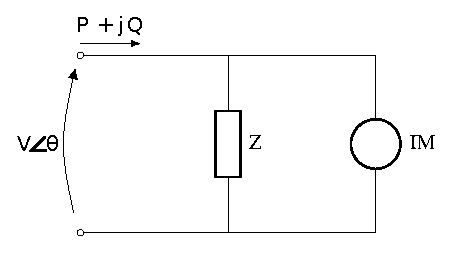
\includegraphics[scale=1]{Images/drawZIM.eps}
    \end{center}
    \label{img: Z-IM}
\end{figure}

\begin{equation}
    \begin{cases}
        \dot{\Delta E'} = \frac{-1}{T_{o}X'}[X\Delta E' + (X - X')V_{0}\sin\delta_{0}\Delta \delta] + \frac{(X - X')\cos\delta_{0}}{T_{0}X'}\Delta V \\
        \\
        \dot{\Delta \delta} = \frac{(X-X')V_{0}}{T_{0}X'E'_{0}}\cdot\left(\frac{\sin\delta_{0}\Delta E'}{E'_0} - \cos\delta_{0}\Delta\delta\right) + \Delta\omega - \frac{(X - X')\sin\delta_0}{T_o X'E'_0}\Delta V \\
        \\
        \dot{\Delta \omega} = \frac{-V_{0}}{MX'}(\sin\delta_{0}\Delta E' + E'_{0}\cos\delta_{0}\Delta\delta) - \frac{E'_0\sin\delta_0}{MX'}\Delta V
    \end{cases}
    \label{eq: xZIM}
\end{equation}

\begin{equation}
    \begin{cases}
        \Delta P = \frac{-V_{0}}{X'}(\sin{\delta_{0}}\Delta E' + E'_{0}\cos{\delta_{0}}\Delta \delta) + \left(2G_{s} V_{0} - \frac{E'_{0} \sin{\delta_{0}}}{X'}\right)\Delta V \\
        \\
        \Delta Q = \frac{-V_{0}}{X'}(\cos{\delta_{0}}\Delta E' + E'_{0}\sin{\delta_{0}}\Delta\delta) + \left(2B_{s} V_{0} + \frac{2V_{0} - E'_{0} \cos{\delta_{0}}}{X'}\right)\Delta V
    \end{cases}
    \label{eq: yZIM}
\end{equation}

\begin{equation}
    \begin{cases}
    X = X_{s} + X_{m} \\
    X' = X_{s} + \frac{X_{m} X_{r}}{X_{m} + X_{s}} \\
    T_{o} = \frac{X_{r} + X_{m}}{\omega_{s} R_{r}}
    \end{cases}
    \label{eq: terms}
\end{equation}

\noindent where the terms $\Delta E'$ and $\Delta \delta$ represent the variation on voltage magnitude and angle at the motor terminals, $\Delta \omega$ is the variation on stator speed, in rad/s. $X_m$, $X_s$ and $X_r$ are the magnetizing, stator and rotor reactances, respectively, $R_r$ stands for the rotor resistance, $\omega_{s}$ is the synchronous speed, $T_o$ represents the open-circuit transient time constant, $M$ is the motor inertia and $V_{0}$ is the voltage on the load terminals before the disturbance. The state, output, input and parameter vectors are presented in \eqref{eq: ZIMstate}, \eqref{eq: ZIMoutput}, \eqref{eq: ZIMinput} and \eqref{eq: ZIMparam}, respectively.

\begin{equation}
	x = [\Delta E', \Delta \delta, \Delta \omega]^{T}
	\label{eq: ZIMstate}
\end{equation}

\begin{equation}
	y = [\Delta P, \Delta Q]^{T}
	\label{eq: ZIMoutput}
\end{equation}

\begin{equation}
	u = [\Delta V]
	\label{eq: ZIMinput}
\end{equation}

\begin{equation}
	p = [X, X', T_{0}, M, G_{s}, B_{s}, E'_{0}, \delta_{0}]^{T}
	\label{eq: ZIMparam}
\end{equation}

The Z-IM load model is much more complex than the spring-mass system, with 9 parameters to be estimated. The hybrid approach proposed was able to estimate the parameters of this system and the comparison between real and modeled behaviour with the parameters obtained can be seen in the Figure \ref{fig: ZIM}.

\begin{figure}[h]
	\caption{Result of parameter estimation for Z-IM Load Model}
	\begin{center}
		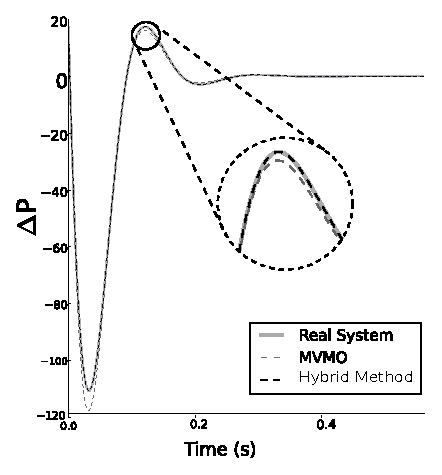
\includegraphics[scale=1]{Images/ZIM.eps}
	\end{center}
	\label{fig: ZIM}
	\legend{Source: \cite{Gomes2019}}
\end{figure}

The application of the hybrid approach on Linearized Z-IM Load Model is subject of a paper presented by the author on the 2019 IEEE Canadian Conference on Electrical and Computer Engineering entitled ``\textit{Load Model Identification Through a Hybrid Approach}".
% ---
\end{apendicesenv}